\documentclass{beamer}

\mode<presentation> {
\usecolortheme{seagull}

\setbeamertemplate{footline}[page number]}
\usepackage{graphicx} 
\usepackage{booktabs} 
\usepackage{url}
\usepackage{hyperref}

\AtBeginSection[]{
  \begin{frame}
  \vfill
  \centering
    \usebeamerfont{title}\Huge{\insertsectionhead\par}
  \vfill
  \end{frame}
}

%-------------------------------------------------------------------------

\title[TLKDCC Memory, Interrupts, Scheduling]{Memory management, Interrupts and Scheduling}
\author{Hans Holmberg}
\institute[LKTP]
{
Linux Kernel Teaching Project \\ 
\medskip
\textit{hans.holmberg@gmail.com}
}
\date{\today}
%------------------------------------------------------------------------
\begin{document}

\begin{frame}
\titlepage

\includegraphics{../common/tux} 
\end{frame}

\begin{frame}
\frametitle{Overview}
\tableofcontents 
\end{frame}

%-----------------------------------------------------------------------
\section{Memory management}

\begin{frame}
\frametitle{Adress types}
\begin{itemize}
	\item \textbf{Virtual addresses:} Regular addresses for userspace programs. May or may not be backed by physical addresses.
	\item \textbf{Physical addresses:} Used between the processor and the systems memory. Not necessarily the same as bus addresses.
	\item \textbf{Bus adresses:} Used between peripheral buses and memory. Can sometimes be remapped with an IOMMU to provide features like making system memory appear as physically contiguous. 
	\item \textbf{Kernel logical adresses:} The regular addresses used in the kernel. Often treated as if they were physical addresses and are mapped to a portion or all of the physical memory. Physical and logical addresses usually only differ by a fixed offset and are linear.
\end{itemize}
\end{frame}

\begin{frame}
\frametitle{Pages frames}
\textbf{Physical memory is grouped into fixed size chunks:}
\begin{itemize}
	\item Each chunk is called a page frame and are numbered sequentially.
	\item The size of page frames can vary but are usually 4096 bytes long.
	\item PAGE\_SIZE is defined to the size of the target you’re building for.
\end{itemize}
\end{frame}

\begin{frame}
\frametitle{Allocating memory in the kernel}
void *kmalloc(size\_t size, gfp\_t flags) \\
The normal method of allocating memory in the kernel.
\textbf{Commonly used flags:}
\begin{itemize}
	\item GFP\_KERNEL: Normal kernel memory. May sleep.
	\item GFP\_ATOMIC: Allocation will not sleep. May use emergency pools. Can be used in interrupt handlers where sleeping is not allowed.
	\item GFP\_DMA: Allocate memory suitable for DMA. Ie. in the lower 32-bit address range
\end{itemize}
\end{frame}

\begin{frame}
\frametitle{Userspace: threads share process memory}
\begin{center}
	\includegraphics[width=3cm]{media/memorymap.pdf}
\end{center}
\end{frame}


%-----------------------------------------------------------------------
\section{Interrupts and scheduling}

\begin{frame}
\frametitle{Concurrency}
Sharing time across multiple processors.
\begin{itemize}
	\item Your code can be interrupted at any time (with a few exceptions).
	\item Your code can be running at the same time on multiple CPUs.
	\item Your code can be re-entered by the same CPU.
	\item Always control access to shared data.
\end{itemize}
\end{frame}

\begin{frame}
\frametitle{Code execution modes}
\begin{itemize}
	\item \textbf{Interrupts:} handle something that needs immediate attention, usually from a piece of hardware. The alternative is polling, which is less efficient.
	\item \textbf{SoftIRQs, Tasklets:} handle something directly, but allow interrupts
	\item \textbf{Kernel threads, user space threads:}
	\begin{itemize}
		\item Kernel threads and users space threads are tasks
		\item System calls are executed in the context of user space task
		\item Kernel threads are used to defer work or handle background task
	\end{itemize}
\end{itemize}
\end{frame}

\begin{frame}
\frametitle{Interrupts}
\begin{itemize}
	\item Is not associated with a kernel process - no current task available.
Cannot sleep.
	\item Is time critical since it interrupts other code.
	\item Try to defer any work to outside of interrupt context).
	\item No access to userspace (copy\_from\_user(), copy\_to\_user(), get\_user(), put\_user())
\end{itemize}
\end{frame}

\begin{frame}
\frametitle{Top and bottom half interrupt handling}
\begin{itemize}
	\item \textbf{Top half:} Do what is absolutely needed in interrupt context (i.e. let the device know that you have received the interrupt)
	\item \textbf{Bottom half:} Process the interrupt and the data that has been delivered
\end{itemize}

Easy to implement with the kernel’s threaded irqs API \footnote{\url{https://www.kernel.org/doc/htmldocs/kernel-api/API-request-threaded-irq.html}\\} \\
Note: you need to use the flag IRQF\_ONESHOT for the pi..

\end{frame}


\begin{frame}
\frametitle{Soft IRQs}
\begin{itemize}
	\item Pending Soft IRQs are executed when when the kernel is about to return to user space.
	\item The Soft IRQs are statically allocated at compile time
	\item Handlers must be reentrant
	\item Only six types in use
	\item Examples: NET\_TX\_SOFTIRQ, NET\_RX\_SOFTIRQ
	\item Efficiently distributes deferred work across CPUs
	\item Good for highly threaded, high frequency tasks
	\item May not sleep
\end{itemize}
\end{frame}

\begin{frame}
\frametitle{Tasklets}
\begin{itemize}
	\item Similar to Soft IRQs, and implemented on top 
	\item All tasklets of the same type is handled sequencially and on the scheduling CPU
	\item Handlers do not  need to be reentrant
	\item May not sleep
\end{itemize}
\end{frame}

\begin{frame}
\frametitle{Work queues}
\begin{itemize}
	\item Queue work in kernel space
	\item Executed by worker thread (kernel task)
	\item Priority can be set.
\end{itemize}
\end{frame}

\begin{frame}
\frametitle{Summary}
\includegraphics[width=0.8\textwidth]{media/interrupts.pdf}
\end{frame}

\begin{frame}
\frametitle{Scheduling}
\textbf{Realtime Scheduling Policy: Each task has a priority}
\begin{itemize}
	\item SCHED\_FIFO: First-in, first-out scheduling algorithm Task continues to run until it blocks or explicitly yields
	\item SCHED\_RR: Each process can run only until it exhausts a predetermined timeslice
	\item SCHED\_DEADLINE: Earliest Deadline First (EDF) scheduling
\end{itemize}
\textbf{Normal Scheduling Policy:}
\begin{itemize}
	\item SCHED\_NORMAL: Completely Fair Scheduler, used for cycles not spent on realtime tasks.
\end{itemize}
\end{frame}

\begin{frame}
\frametitle{SCHED\_NORMAL: completely fair scheduler}
\begin{itemize}
	\item Tries to emulate a processor that is capable of running several tasks simultaneously.
	\item Aims to compensate a task for the time it has not been running, by calculating the wait time. 
	\item When a task is running, it the wait time decreases and eventually a task with a longer wait time is scheduled.
\end{itemize}
See the kernel documentation for more information.\footnote{Kernel documentation, CFS scheduler \url{http://lxr.free-electrons.com/source/Documentation/scheduler/sched-design-CFS.txt} \\}

\end{frame}
%-----------------------------------------------------------------------

\begin{frame}
\Huge{\centerline{Thanks!}}
\end{frame}

\end{document} 
